%# -*- coding: utf-8-unix -*-
%%==================================================
%% chapter01.tex for SJTU Master Thesis
%%==================================================

%\bibliographystyle{sjtu2}%[此处用于每章都生产参考文献]
\chapter{前言}
\label{chap:preli}


\section{机器学习}

机器学习是一种赋予计算机学习能力,并让它完成直接编程无法完成的功能的方法。从实践角度讲,机器学习方法是利用已有的数据,得出某种模型,并利用此模型做预测的一种方法。机器学习可以视为模仿人类思考模式的过程。人类通过学习,积累知识经验,归纳生活规律。当人类遇到位置的问题或对未来进行推测时,就可以使用这些经验规律进行推测。机器学习中的“训练”和“预测”即对应人类的“归纳”和“推测”。

机器学习涉及的范围非常广阔。机器学习的基础包括概率论、数理统计、线性代数等。同时,机器学习可以作为工具,和其他领域的各种技术相结合,形成众多的交叉学科,包括数据挖掘、计算机视觉、语音识别技术、自然语言处理等。数据挖掘是利用机器学习处理海量数据的能力,从大量的数据中发现具有价值的东西;计算机视觉是机器学习与图像处理的结合,图像处理技术将图像处理为适合机器学习算法的输入,然后机器学习从图像中进行识别操作,例如手写识别等;语音识别技术是音频处理技术和机器学习的结合,例如苹果公司的Siri等;自然语言处理是让机器理解人类语言的学科,涉及词法分析、语法分析等编译相关的知识,是机器学习分类中备受瞩目的一个分支。

机器学习的算法种类五花八门。其中最为重要的算法主要分为以下几种类型:

\begin{enumerate}
	\item [(1)] \textbf{回归算法(Regression)}:代表为线性回归(Linear Regression)和逻辑回归(Logistic Regression)。线性回归指寻找一条直线可以最好地拟合数据,主要思想是最小二乘法。逻辑回归与线性回归相似,但线性回归的目标是预测一个数值,逻辑回归的目标是判断二分类。逻辑回归的主要思想是Sigmoid函数。
	\item [(2)] \textbf{神经网络(Neural Networks)}:神经网络本质是计算机模拟大脑的思考过程。神经网络对数据进行分解,由一层层的“神经元”处理数据,并把处理后的数据送给下一层神经元。每一个神经元都是一个逻辑回归模型,众多的神经元按层级结构组合起来,可以处理非常复杂的分类问题。神经网络的一个典型的应用就是手写数字识别问题(MNIST)。
	\item [(3)] \textbf{支持向量机(Support Vector Machine, SVM)}:SVM是对逻辑回归的优化,可以比逻辑回归更好地划分分类线。而且通过与核(Kernel)函数的结合,SVM可以在低维空间表达出高维空间的分类界限,在保留原本计算复杂性的条件下大大增强了分类的准确度。
	\item [(4)] \textbf{聚类算法}:前三类算法的基本条件是训练数据是有标签的数据,在训练后可以对同类型未标签的数据进行预测。而聚类算法是应用于无标签数据集上的算法,作用是计算数据群体中互相的间距,并根据间距的大小将数据划分为多个类别。K-Means算法就是典型的聚类算法。
\end{enumerate}

除了上述列出的算法以外,机器学习领域还有诸如用于决策的增强学习(Reinforcement Learning)、多隐藏层神经网络的深度学习(Deep Learning)等大型分支。机器学习是目前最火热的计算机科学领域之一。从AlphaGo到智能车自动驾驶,从谷歌识图到微软小冰,机器学习的实践应用也屡屡让世界惊叹。



\section{网络诈骗中的分类算法}

网络诈骗有多种类型,例如网页诈骗 \cite{Spirin:2012}、邮件诈骗 \cite{Castillo:2007}、远程通信诈骗 \cite{Yao:2017}和概念诈骗 \cite{Jindal:2008}。水军检测问题属于概念诈骗领域。面对这类问题,早期研究者们热衷于使用NLP和数据挖掘技术对各种概念进行分类和总结。后来他们试图优化文本分析方法,Shojaee等人 \parencite{Shojaee:2013}认为关注水军评论内容的词法特征和语法特点很关键。由于水军们试图模仿正常评论的内容来隐藏水军评论,所以他们的写作风格和用词风格一直在变化。因此,如果从文体形式出发来考虑的话,就可以辨别出水军评论的相似性,进一步找到那些虚假评论。他们提取出这些特征后使用经典的分类算法和进行检测。Chen等人 \parencite{Chen:2013}提出了基于语义分析的方法,用拆句子工具将评论内容拆分为一个个单词,并通过计算不同评论内容拆分后单词的相似数来衡量语义的相似程度。他们也尝试了使用非监督学习的方法进行检测,但效果并不是很好。

抛开NLP方法,在机器学习方法的帮助下,水军检测问题可以被视为二分类问题或排名问题。其中的关键部分便是特征的选取和模型的选取。可以在水军检测中应用的经典机器学习分类算法有很多:Ott等人 \parencite{Ott:2011}提出了SVM和单词条/双词条文本分析的结合,Chen等人 \parencite{CHEN:2009}提出了朴素贝叶斯NB(Naive Bayes)在文本分类问题中的应用。也有许多研究者在经典方法的基础上进行了改进,并提出了新的方法。Li等人 \parencite{Li:2014}提出了PU(Positive-Unlabeled)学习方法。他们认为在网络平台的过滤系统作用下,那些被过滤系统过滤掉的评论一定是虚假评论,然而被过滤系统判定为正常的评论中却还混有大量的虚假评论。故PU学习适用的数据集是那些只部分标记了一种类型数据,其他数据视为未标记数据的情况。他们还与大众点评公司合作,取得了珍贵的数据,在此基础上提出了新颖的模型。Chino等人 \parencite{Chino:2017}利用用户发布评论的时间间隔和评论内容量特征,训练了一个对数分布模型来拟合大众的特征分布情况,然后找到那些与主流分布隔离开来的点视作可疑用户。寻找与大众情况相异用户的思路非常新颖。Chen等人 \parencite{Chen:2017}提出了一个利用目标排名变动情况来寻找可疑用户的模型。如果目标短时间内在排行榜上发生了大幅震荡——排名迅速上升几天后又迅速下跌——那目标很可能雇佣了水军帮助他增长排名。不仅如此,他们还利用这一点进一步分析,成功捕捉到了水军团队。



\section{隐马尔可夫模型}

隐马尔可夫模型HMM(Hidden Markov Model)是一种经典的概率图模型。如图~\ref{fig:hmm},HMM可以用图来表示各个变量之间的关联。HMM有两个状态:观测态(图中$X_1 \cdots X_n$)和隐藏态(图中$Y_1 \cdots Y_n$)。隐藏态变量$Y_i$形成序列结构,然后每个隐藏态变量$Y_i$生成一个观测态变量$X_i$。在初始化时,HMM有一个初始状态概率(Initial State Probability)来决定由哪种隐藏态开始构建序列。之后每次出现一个新状态,隐藏态序列就增加一个变量,并且变量的值遵循一个特定的转移概率(Transition Probability)。隐藏态变量生成观测态变量的过程也遵循一个特定的输出概率(Emission Probability)。为了保证序列本身和各种概率的的合理性,HMM遵循两个重要的假设:
\begin{enumerate*}		
	\item[(1)] 每一个隐藏态变量的生成都只依赖于它之前的那一个隐藏态变量;
	\item[(2)] 每一个观测态变量的生成都只依赖于它对应的那个隐藏态变量。
\end{enumerate*}
这两个假设在大量的实践中被广泛认可。它们在不对结果产生重大影响的前提下大大简化了模型的计算复杂度。并且它们也保证了转移概率和输出概率的合理性。综上可知,一个特定的HMM序列可以由三个概率表示:初始状态概率、转移概率和输出概率。

\begin{figure}[htbp]
	\centering
	\begin{minipage}[htbp]{0.6\textwidth}
		\centering
		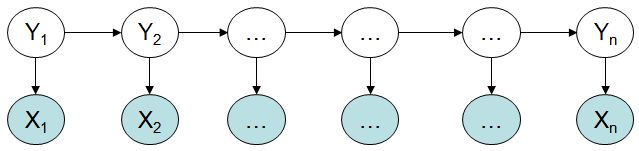
\includegraphics[width=10cm]{preli-1.jpg}
		\caption[HMM示例图]
		{HMM示例图\label{fig:hmm}}		
	\end{minipage}     
\end{figure}

用HMM解决的问题主要有三个类型:

\begin{enumerate}		
	\item[(1)] \textbf{参数估计}:给定一个观测序列,计算一组参数(三个概率)使该观测序列出现的可能性最大;
	\item[(2)] \textbf{由观测态序列确定隐藏态序列(解码问题)}:已知HMM模型,给定一个观测序列,求解最可能的隐藏序列;
	\item[(3)] \textbf{求解观测序列出现的概率}:已知HMM模型,给定一个观测序列,计算该序列出现的概率。
\end{enumerate}

参数估计问题可以视作HMM的训练问题。Rabiner在1989年提出了一种名为\emph{Baum-Welch}\cite{Rabiner:1989}的EM(Expectation-Modification)算法,利用极大似然估计方法来训练HMM参数,现在已经成为了该问题的普遍解决策略。由观测态序列确定隐藏态序列的问题在语音识别领域也称作解码问题,目标是在给定观测序列的情况下寻找概率最高的隐藏序列。Forney在1973年提出来了解决这种问题的\emph{Viterbi}\cite{Forney:1973}算法。计算观测序列概率的问题是计算特定HMM生成特定观测序列的概率。换句话说,这个问题可以用来计算观测序列和给定模型的关联程度。


